\chapter{Bakgrunn}
\label{ch:background}
Første delkapittel gir en innføring i velferdsteknologi, og tegner opp linjene for hvordan veien har gått
fra Hagen-utvalget til utprøving av avstandsoppfølging i kommunene (delkapittel \ref{sec:remotemonitoring}).
Videre blir personvern i helse- og velferdsteknologi kort drøftet med utgangspunkt i Datatilsynet sine retningslinjer
og den nye personvernsforordningen til EU. De to siste delkapitlene handler om \gls{iot} med vekt på hvordan
denne plattformen legger til rette for en ny teknologistakk, og til slutt kort om bruken av \gls{iot} i velferdsteknologi.

\section{Velferdsteknologi}
\citet{regjeringen_hagen} er en norsk offentlig utredning (NOU) om velferdsteknologi med tittelen «Innovasjon i omsorg».
Utredningen benytter følgende definisjon av velferdsteknologi:

\blockquote{
Med velferdsteknologi menes først og fremst
teknologisk assistanse som bidrar til økt trygghet,
sikkerhet, sosial deltakelse, mobilitet og
fysisk og kulturell aktivitet, og styrker den
enkeltes evne til å klare seg selv i hverdagen til
tross for sykdom og sosial, psykisk eller fysisk
nedsatt funksjonsevne. Velferdsteknologi kan
også fungere som teknologisk støtte til pårørende og
ellers bidra til å forbedre tilgjengelighet,
ressursutnyttelse og kvalitet på tjenestetilbudet.
Velferdsteknologiske løsninger kan i
mange tilfeller forebygge behov for tjenester
eller innleggelse i institusjon.
}

\citet{regjeringen_hagen} anbefaler fem punkter for myndighetene å fokusere på i fremtiden:

\begin{enumerate}
    \item «Næromsorg» -- den andre samhandlingsreformen: mobiliser ressurser i samarbeid med
    lokalsamfunnet, det sosiale nettverket til pasienten og familien.
    \item «Teknoplan 2015» -- teknologistøtte til omsorg: bruk ny og eksisterende teknologi for å gi brukere
    bedre trygghet og muligheten til å bo hjemme og motta støtte.
    \item «Nye rom» -- fremtidens boligløsninger og nærmiljø: boliger og leiligheter må tilpasses eldre.
    \item Et nasjonalt program for kommunal innovasjon i omsorg: kommunene har hovedansvaret for omsorgstjenester,
    og myndighetene kan støtte kommunene med incentiver til nye løsninger.
    \item Omsorgsfeltet som næring: Norge kan være en ledende nasjon i utviklingen av nye omsorgsprodukter, og
    eksportere disse innovasjonene. Omsorgsfeltet åpnes opp for importering av eksportering av varer og tjenester.
\end{enumerate}

«Teknoplan 2015» legges fram som en trinnvis plan på tre punkter der punkt én handler om å «videreutvikle trygghetsalarmen
til en trygghetspakke som inkludere tilrettelegging for smarthus» , punkt to handler om å ta i bruk moderne
kommunikasjonsteknologi og sosiale medier for å redusere ensomhet og punkt tre handler om å «ta i bruk teknologi
som stimulerer, underholder, aktiviserer og strukturer hverdagen» \citep[s. 17]{regjeringen_hagen}.

Myndighetenes rolle blir å tilrettelegge for kommunal innovasjon i omsorgssektoren med et nasjonalt program
som kan gi støtte i form av penger og opplæring. \citet[s. 19]{regjeringen_hagen} mener at at det må
etableres en kommunal innovasjonsskole i samarbeid med KS for ledere og andre omsorgspersoner, og at minst én prosent
av budsjettet i omsorgssektoren skal gå til forskning, utvikling og innovasjon.

Stortingsmeldingen «Morgendagens omsorg» bygger på arbeidet til Hagen-utvalget \citep{morgendagens_omsorg}.
I denne meldingen legger regjeringen frem «Omsorgsplan 2020» som inkluderer et program for velferdsteknologi de neste årene.
Ett av initiativene i programmet er å bygge og etablere åpne velferdsteknologistandarder. Dette vil lette integreringen av nye
løsninger i privat og offentlig sektor. Andre initiativer er å utvikle og teste velferdsteknologiløsninger i kommunene,
bygge og dele kunnskap og lage modeller og rammeverk som andre kan bruke.

I revidert statsbudsjett for 2014 bevilget Stortinget penger til et nasjonalt velferdsteknologiprogram. De fem prioriterte
initativene i programmet er:

\begin{enumerate}
    \item Trygghet og mestring hjemme
    \item Avstandsoppfølging av personer med kroniske sykdommer
    \item mHelse
    \item Sosiale nettverk -- motvirke og redusere ensomhet blant eldre
    \item Bidra til økt aktivitet (inkl. fritidsaktiviteter) for barn og unge med nedsatt funksjonsevne
\end{enumerate}

\textquote[\cite{ehelse_mhelse}]{mHelse, eller personlige mobile helseløsninger, er å benytte mobilbaserte verktøy og helseapplikasjoner
(helse-apper) til helseformål}{.}
De ulike initiativene går litt inn i hverandre. Avstandsoppfølging kan føre til mer trygghet og mestring hjemme
og ta i bruk mHelse. Avstandsoppfølging er dekket nærmere i delkapittel \ref{sec:remotemonitoring}.

\section{Avstandsoppfølging av kronisk syke}
\label{sec:remotemonitoring}
\citet{rojahn2016remote} definerer avstandsoppfølging som \textquote{overvåking av en poliklinisk pasient
med en enhet som overfører data}{.}
I avstandsoppfølging følges pasienter opp i sitt eget hjem, og
målet med avstandsoppfølging er å unngå sykehusinnleggelse ved å oppdage forverringer tidlig og la
pasientene behandle sin egen sykdom. Innleggelse på sykehus koster gjennomsnittlig 40000 kr per døgn og er en stor utgift
for helsemyndighetene \citep{regjeringen_innleggelse}.

Kroniske sykdommer er den mest vanlige dødsårsaken på verdensbasis \citep{who_chronic}.
I følge \citet{austad2016sensorer}, kan kroniske sykdommer som KOLS, hjerte- og karsykdommer og diabetes
følges opp klinisk med noen få sensorer: vekt, blodtrykksmåler, pulsoksymeter og spirometer. Typiske
tegn på hjertesvikt kan være tungpusthet, vektforandring, hoste, hjertebank, hevelser i beina og
tretthet/tiltaksløshet \citep{ehelse_hjertesvikt} \citep{nasjonalforeningen}.

Fire kommuner ble valgt ut til å ta del i et nasjonalt prosjekt for å legge til rette for økt mestring
og trygghet hjemme med nye digitale behandlingsmetoder: Trondheim kommune, Stavanger kommune, Oslo kommune og Sarpsborg kommune.
Stortinget bevilget 30 millioner som en del av budsjettavtalen for 2015 til prosjektet som omfatter rundt 4-500 brukere. %@TODO:
%https://www.regjeringen.no/no/aktuelt/nye-digitale-behandlingsmetoder-for-personer-med-kroniske-sykdommer/id2414937/
Her er de første forskningsresultatene ventet i midten av 2017. Foreløpige resultater fra Oslo kommune viser at
en klar reduksjon i bruken av sykehustjenester (færre konsultasjoner og innleggelser), samt nedgang i bruk av
tjenester fra hjemmesykepleien. Den viser også besparelser på 73000 kr i gjennomsnitt hvert år (reduksjon på 32\%).
% @TODO kilde? https://helsedirektoratet.no/nyheter/bedre-kvalitet-med-velferdsteknologi-i-helse-og-omsorgstjenestene for når forskningsresultatene er ventetn
% @TODO kilde? for det siste her: https://www.regjeringen.no/no/aktuelt/velferdsteknologi-bidrar-til-bedre-hverdagshelse/id2483590/
% http://www.ks.no/contentassets/7f30e3e8219b425484c885a3ee0dcd41/une-tangen.pdf

%\section{Eldre pasienter og IT}
\section{Personvern i helse- og velferdsteknologi}
For velferdsteknologi spesielt, oppgir \citet{datatilsynet_welfare} ti viktige generelle retningslinjer for å sikre personvernet
i utviklingen av ny velferdsteknologi:

\begin{enumerate}
    \item Velg den minst inngripende løsningen
    \item Begrens mengden data som lagres
    \item Velg sanntidsløsning hvis mulig
    \item Lagre lokalt hvis mulig
    \item La brukeren ha kontroll over løsningen
    \item Slett data etter bruk
    \item Begrens tilgangen til informasjon
    \item Innsyn i egne data
    \item Dataene bør krypteres
    \item Anonymisering av data
\end{enumerate}

En ny personsvernsforordning ble vedtatt av EU 27.april i år. Denne overtar
etter personverndirektivet som er implementert i norsk lovgivning gjennom
personopplysningsloven. Forordningen trer i kraft 25. mai 2018, og medfører
strenge sanksjoner til selskaper som bryter reglene. Siden Norge er et EØS-medlem,
må hele forordningen tas inn i det norske lovverket.

\citet{datatilsynet_privacy} skriver at \textit{innebygd personvern} betyr at det tas hensyn
til personvernet i alle utviklingsfaser av et system eller en løsning. Det er
både kostnadsbesparende og mer effektivt enn å endre et ferdig system. Innebygget
personvern er tatt med i den nye personvernforordningen til EU.
Artikkel 25 sier at standarden til et system skal være at man kun prosesserer
og lagrer de personopplysningene som skal til for å løse de oppgavene
systemet har (Council of European Union, 2016).
%http://eur-lex.europa.eu/legal-content/en/TXT/?uri=CELEX:32016R0679

Artikkel 7 i forordningen har tittelen Vilkår for samtykke. Selskapet må
innhente eksplisitt samtykke, samt vise at det har hentet inn et slikt samtykke.
Samtykket må vise hva slags informasjon som samles inn, og hva informasjonen
skal brukes til. Et viktig moment her er at dette samtykket skal kunne
trekkes tilbake når som helst på en enkel og brukervennlig måte (Council of
European Union, 2016).

Det siste viktige punktet i forordningen er den korte fristen fra man oppdager
et datainnbrudd til man varsler den relevante myndigheten. Denne fristen er
satt til 72 timer. Merk at man ikke nødvendigvis må varsle offentligheten. Om
myndigheten tror at innbruddet vil gå ut over individuelle brukere må disse
bli varslet av selskapet (Berntsen, 2016).
%Berntsen, J. (2016). Compliance: general data protection regulation. Hentet
%17. desember 2016
%http://docplayer.me/24846608-Compliance-general-data-protection-regulation-johnny-berntsen-iso-iec-master-knowit.html

Personvernsforordningen inneholder hjemler for å straffe selskap som bryter reglene.
I verste fall kan et selskap få 20 millioner euro i
bot, eller opptil 4 \% av fjorårets globale omsetning.
Mildere sanksjoner er skriftlige advarsler, og periodiske
granskninger av datasikringen (Wikipedia, 2016b).
%https://en.wikipedia.org/w/index.php?title=General_Data_Protection_Regulation&oldid=754575179

\textbf{TODO:} Legge inn noe om at helsedata må lagres i Norge? Og om debatten om outsourcing som har vært i det siste?
Pluss kanskje noe om tofaktorautentisering? Hvordan sette strek?

%Datalagring. det med å sette tjenester til utlandet

\section{Tingenes internett (IoT)}
\citet{iot_legal} definerer tingenes internett som en
\textquote{fremvoksende global Internett-basert informasjonsarkitektur som
fasiliterer utvekslingen av varer og tjenester}{.} I denne definisjonen ligger det en
visjon om en verden knyttet sammen av objekter som kommuniserer med hverandre.

Andre definisjoner av \gls{iot} eksisterer avhengig av bransje. \citet{iot_harvard_smart} skriver
at tingenes internett ikke er en veldig god beskrivelse av den nye trenden med
sammenkoblete enheter: 
\textquote{Det som gjør smarte, tilkoblede produkter fundamentalt annerledes er ikke Internett,
men at «tingenes» natur endrer seg. Det er de nye mulighetene til smarte, tilkoblede produkter
og dataen de genererer som fører til en ny periode med konkurranse}{.}

Derfor introduserer de begrepet «smarte produkter» som består av tre elementer:

 \begin{itemize}
    \item Fysiske komponenter: de elektriske og mekaniske delene til produktet.
    \item «Smarte» komponenter: sensorer, prosessorer, programvare, operativsystem, lagring, brukergrenesnitt.
    \item Tilkoblingskomponenter: porter, antenner, protokoller som muliggjør kablede/trådløse tilkoblinger
    én-til-én, én-til-mange, mange-til-mange.
\end{itemize}

Smarte produkter introduserer en ny teknologistakk (figur \ref{fig:iot_harvard_smart}) med produkter koblet til
en produktsky. Produktskyen inkluderer et «Big Data»-databasesystem og regel- og analysemotor for å håndtere
forretningslogikk på en effektiv måte, og utnytte og analysere all informasjonen fra produktene.
Disse smarte, tilkoblede produktene har fire egenskaper som bygger på hverandre: Overvåking, kontroll,
optimalisering og autonomi. Tesla er et eksempel på et smart produkt som kombinerer overvåking, kontroll og
optimalisering for å oppnå autonomi. Bilen diagnoserer seg selv, og oppdaterer seg selv automatisk uten
at den må på verksted.

\citet{iot_harvard_smartcompanies} antyder at smarte, tilkoblede produkter endrer selskaper også, ved
å endre hvert steg i verdikjeden. Utnyttelse av data blir mer viktig, og produktdesign er ikke bare noe
mekanisk, men et tverrfaglig samarbeid der programvareutvikling vil spille en større rolle. 

\begin{figure}
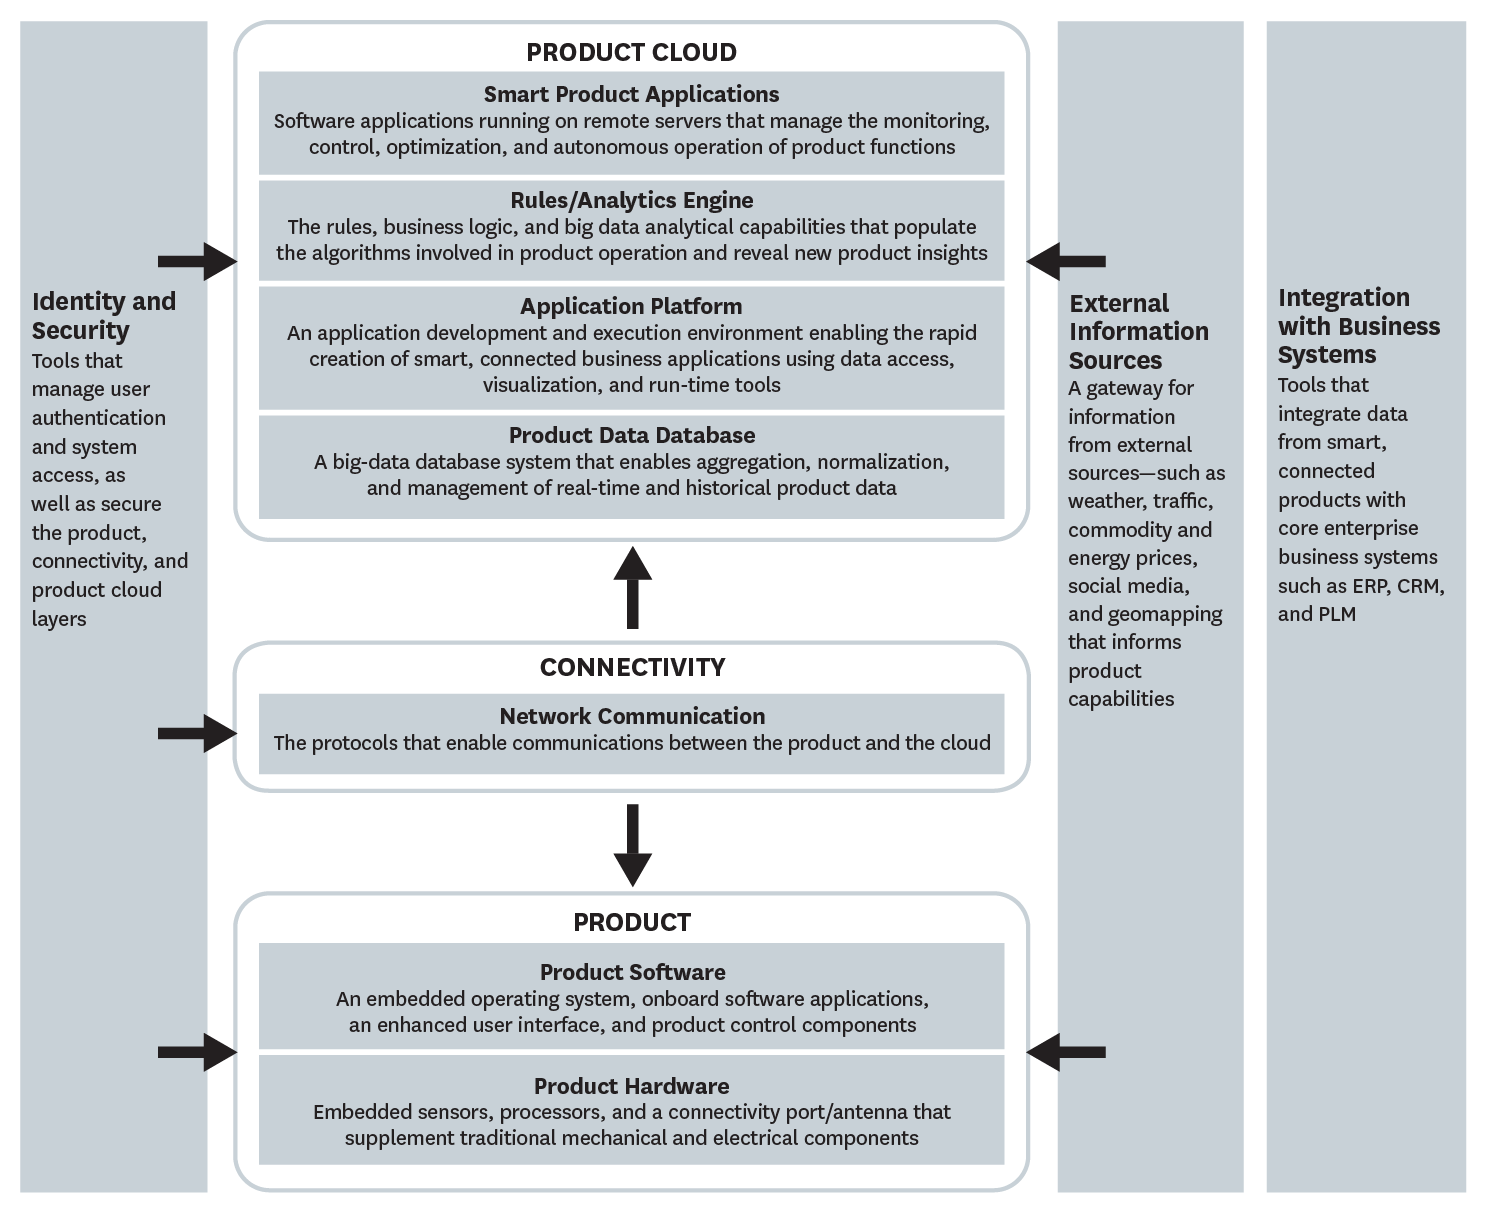
\includegraphics[width=1.1\textwidth,center]{fig/harvard_technology}
\caption{Den nye teknologistakken \citep{iot_harvard_smart}.}
\label{fig:iot_harvard_smart}
\end{figure}

\begin{figure}
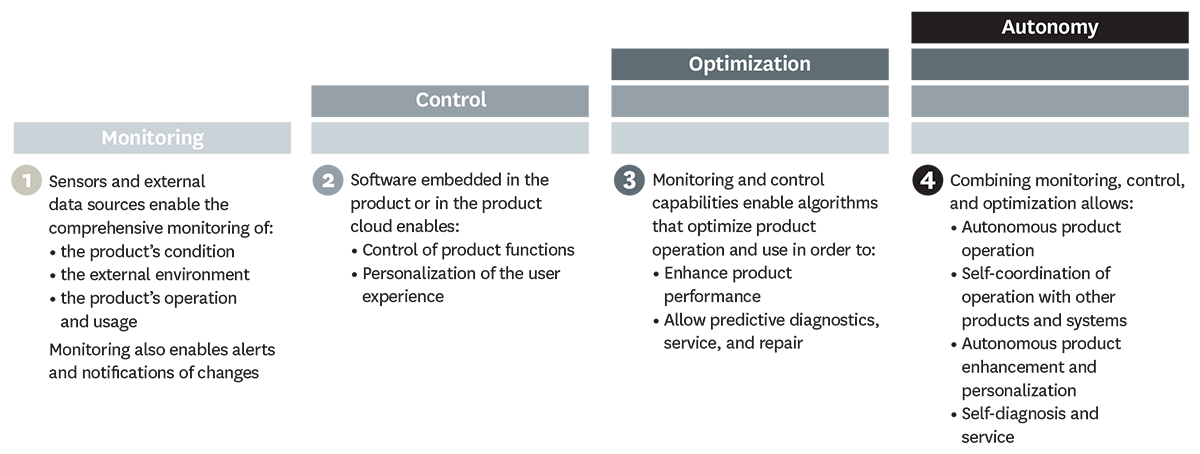
\includegraphics[width=1.1\textwidth,center]{fig/harvard_capabilities}
\caption{Egenskapene til smarte produkter \citep{iot_harvard_smart}.}
\label{fig:iot_harvard_capabilities}
\end{figure}


\subsection{Sikkerhet i tingenes internett}
Eksperter har kommet med innvendinger når det gjelder sikkerhetsmodellen til \gls{iot}.
21. oktober 2017 ble Internett-kjerneinfrastrukturselskapet \textit{Dyn} angrepet via flere millioner
små enheter (hovedsaklig rutere og kameraer) med lav grad av sikkerhet \citep{iot_attack_ddos}.
Dette påvirket flere store nettsider som Twitter, Spotify og PayPal. Rutere og webkameraer leveres
ofte med standardpassord som brukere ikke endrer selv. I tillegg til dette kan flere vanlige
porter som 22 (SSH), 80 (HTTP) og 23 (Telnet) være helt åpne mot omverdenen \citep{iot_mirai_botnet}.

\citet{iot_schneier_regulation} oppfordrer myndighetene til å pålegge restriksjoner på \gls{iot}.
Han argumenterer for at markedene selv ikke klarer å beskytte sikkerheten til forbrukerne.
Forbrukerne bryr seg ikke, produsentene bryr seg ikke og produktene kan aldri patches
etter de er solgt og levert. Denne diskusjonen om reguleringer må gjøres før det skjer
en \gls{iot}-katastrofe, mener Schneier. % @Todo: en iot-katastrofe where feelings are heated?


\section{Tingenes internett i velferdsteknologi}
Personal Connected Health Alliance (PCHA) publiserer Continua-designretningslinjene hvert år,
et åpent rammeverk for ende-til-ende-kompabilitet i personlige, tilkoblede helseenheter og helsesystemer \citep{continua_guidelines}.
En oversikt av Continua-rammeverket kan finnes i figur \ref{fig:continua}. Personlige enheter kommuniserer med
protokoller som Bluetooth eller Zigbee til en hub (Personal Area Network), og denne huben sender informasjonen
videre til et telehelse-servicesenter. Derfra kan dataen overføres til helseregisteret.

Som en del av «Omsorgsplan 2020» og nasjonalt program for velferdsteknologi, bestemte regjeringen
i slutten av 2014 at Continua-rammeverket skal være grunnlaget for alle velferdsteknologiløsninger i Norge.
Dette var også anbefalingen til Helsedirektoratet --
å standardisere på ett rammeverk sikrer at ulike løsninger virker godt sammen \citep{regjeringen_continua}.

\begin{figure}
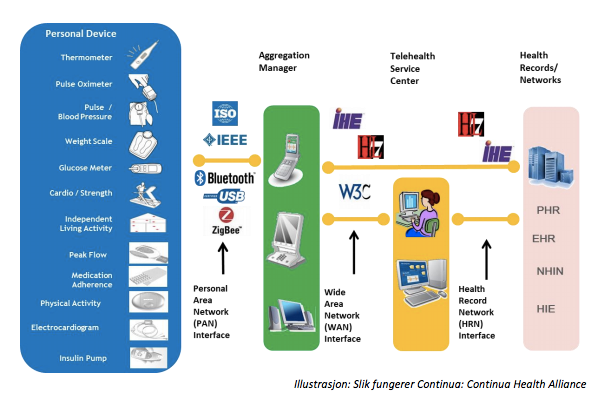
\includegraphics[width=0.9\textwidth,center]{fig/continua}
\caption{Oversikt over Continua-rammeverket}
\label{fig:continua}
\end{figure}
